\documentclass[11pt,a4paper]{article}

\usepackage[T1]{fontenc}
\usepackage[utf8]{inputenc}
\usepackage{lmodern}
\usepackage{microtype}
\usepackage[margin=2.4cm]{geometry}
\usepackage{amsmath,amssymb}
\usepackage{booktabs}
\usepackage{tabularx}
\usepackage{xcolor}
\usepackage{tikz}
\usetikzlibrary{arrows.meta,positioning,fit,calc}
\usepackage{pgfplots}
\pgfplotsset{compat=1.18}
\usepackage[numbers,sort&compress]{natbib}
\usepackage{hyperref}
\hypersetup{colorlinks=true,linkcolor=teal!60!black,citecolor=teal!60!black,urlcolor=teal!60!black}
\usepackage{caption}
\captionsetup{font=small,labelfont=bf}

\definecolor{qkteal}{HTML}{1F6F78}
\definecolor{qkgrey}{HTML}{9AA3AB}
\definecolor{qkred}{HTML}{B4432F}

\newcommand{\qk}{QuipKeys}
\newcommand{\ttw}[1]{\texttt{#1}}

%% Numbers from the held-out benchmark (filled from qk-bench output).
\newcommand{\ModFix}{77.3}
\newcommand{\ModFixPlain}{53.5}
\newcommand{\BlindNone}{?}
\newcommand{\BlindAcc}{?}


\title{\qk: Decoding Imprecise Physical-Keyboard Typing\\with a Context-Aware Noisy-Channel Model}
\author{Hasnat\\[2pt]\small\url{https://github.com/codinghasnat/quipkeys}}
\date{November 2026}

\begin{document}
\maketitle

\begin{abstract}
Phone keyboards stopped asking for precision years ago: they decode where a finger probably meant to land. Physical keyboards never made that transition, and desktop autocorrect remains a conservative dictionary spellchecker. We present \qk{}, an offline decoder for physical-keyboard typing that aims to let people type fast and imprecisely, without looking and without reaching for backspace, and still get the words they intended. \qk{} combines a keyboard-geometry error model, a weighted edit-distance search over a dictionary trie, an interpolated trigram language model built from 1.4 billion words of text, and a sliding-window lattice decoder whose confidence is the posterior probability of each correction summed over all decoding paths. Safety mechanisms (name and code protection, a morphology guard, hysteresis, undo-driven learning) keep false corrections to about one in 750 correctly typed words. Beyond letter slips, it repairs misplaced spaces, whole-hand shifts, Shift-key slips and accidental Caps Lock.

On a held-out benchmark of simulated sloppy typing, \qk{} fixes \ModFix\% of mistyped words at moderate error rates (a frequency-only spellchecker: \ModFixPlain\%) and lifts word accuracy for ``blind'' typing (10\% of letters wrong) from \BlindNone\% to \BlindAcc\%. In a first real-typing study with one participant typing 33 passages at a median of 85~words per minute with the text hidden and backspace disabled, words typed exactly right rose from 75.4\% to 91.5\% (92.5\% with an error model fitted to the participant), and the held-out half of the data shows the gains generalise. The real data also overturned two assumptions the simulator had baked in: this typist's extra letters are rarely neighbouring keys, so keyboard geometry contributed nothing on real typing, and swapped letters happen at normal speed rather than as fast roll-overs. We release the engine, benchmark and data-collection tools, and discuss what remains before such a decoder could replace autocorrect.
\end{abstract}

\section{Introduction}

Typing accurately on a physical keyboard is slow. Skilled typists spend a large share of their keystrokes on correction: noticing an error, backspacing over it, retyping. Large-scale keystroke studies show that corrections are a substantial part of everyday typing, even for fast typists~\citep{dhakal2018}. The cost is not only the keystrokes. Watching for errors pulls attention from what one is writing.

Touchscreen keyboards solved a harder version of this problem. A finger on glass has no tactile boundary between keys, so phone keyboards treat each tap as noisy evidence and decode the intended word with a language model~\citep{goodman2002,kristensson2004,vertanen2015}. Users learned they can type sloppily on a phone and mostly get the right words. Physical keyboards never got that treatment. Desktop autocorrect, in the operating system or the word processor, is still a cautious dictionary spellchecker. It fixes \ttw{teh}, but it does not reason about which key a finger probably meant, it rarely uses context, and it does not repair misplaced spaces.

\qk{} asks what happens if a physical keyboard gets a real decoder. Our north star is a typist who does not care where their fingers land. There is still intent, but each key press lands only roughly near the intended key, and the typist never looks down or backspaces. The metric that matters is not spelling accuracy but \emph{effective words per minute}: correct words produced per minute, after all corrections.

\paragraph{Contributions.}
\begin{enumerate}
\item A complete offline decoder for physical-keyboard input (\S\ref{sec:system}). It runs in a few milliseconds per word in pure Rust: a geometry- and timing-aware error model, a weighted trie search, an interpolated trigram language model, and a sliding-window lattice decoder with path-summed confidence.
\item A set of safety mechanisms aimed at the failure that makes people turn autocorrect off: changing what they meant to type (\S\ref{sec:safety}).
\item Handling of error types that word-level spellcheckers do not see: misplaced and missing spaces, whole-hand shifts, Shift-key slips and accidental Caps Lock (\S\ref{sec:special}).
\item A benchmark with a simulated sloppy typist at five error levels, including a ``rough aim'' model in which every press is Gaussian-distributed around the intended key (\S\ref{sec:eval}).
\item A first real-typing evaluation: 33 passages from one participant, with error-profile analysis that exposed where the simulator was wrong (\S\ref{sec:real}).
\end{enumerate}

\section{Related Work}

\paragraph{Spelling correction.} Edit distance~\citep{damerau1964,levenshtein1966} underlies most spelling correction. The noisy-channel formulation~\citep{kernighan1990,brill2000} chooses the intended word $w$ that maximises $P(t\mid w)\,P(w)$ for typed string $t$. Real-word errors, typos that happen to produce another valid word, need context, and were addressed early with $n$-gram models~\citep{mays1991}. SymSpell~\citep{garbe2012symspell} popularised fast candidate generation by symmetric deletion. These systems model cognitive misspellings (\ttw{recieve}) at least as much as motor slips, and they correct one word at a time.

\paragraph{Decoding touch input.} Soft-keyboard work combined key-press likelihoods with language models from early on~\citep{goodman2002}. Shape writing decodes whole gestures~\citep{kristensson2004}, and VelociTap showed that decoding whole sentences of very imprecise taps supports fast and accurate entry~\citep{vertanen2015}. Our lattice decoder follows the same principle, applied to discrete key events from a physical keyboard, where the only spatial evidence is \emph{which} key fired.

\paragraph{Typing behaviour and data.} Large keystroke datasets~\citep{dhakal2018} and corpora of real typos~\citep{hagiwara2020} document how people mistype. We could not access these in our build environment, which is one reason our real-typing study collects its own keystroke logs.

\section{System}
\label{sec:system}

Figure~\ref{fig:pipeline} shows the pipeline. Text arrives as a stream of typed chunks separated by spaces, each with per-key timestamps. Every chunk is decided when its space is pressed, so corrections appear immediately. The recent chunks are also re-decoded jointly as more context arrives.

\begin{figure}[t]
\centering
\resizebox{\linewidth}{!}{%
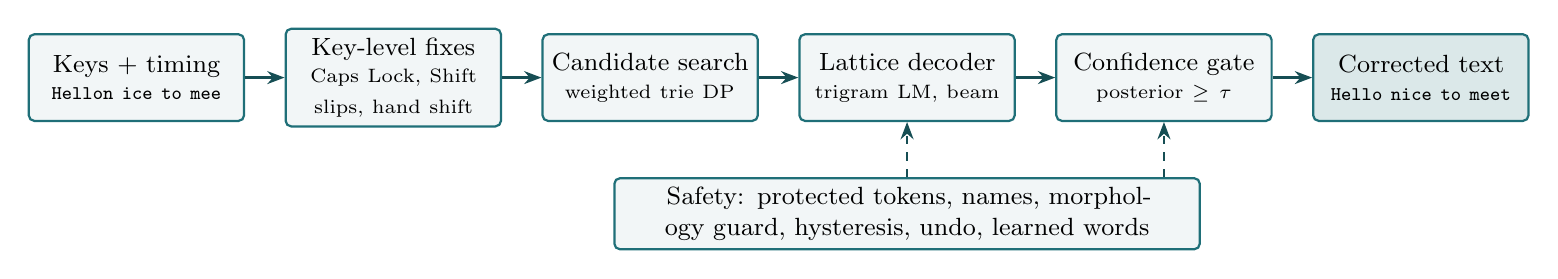
\begin{tikzpicture}[
  box/.style={draw=qkteal,rounded corners=2pt,thick,fill=qkteal!6,align=center,font=\small,minimum height=1.1cm,text width=2.5cm},
  arr/.style={-{Stealth[length=2.2mm]},thick,qkteal!70!black},
  node distance=0.5cm]
\node[box] (in) {Keys + timing\\[-1pt]\scriptsize\ttw{Hellon ice to mee}};
\node[box,right=of in] (pre) {Key-level fixes\\[-1pt]\scriptsize Caps Lock, Shift slips, hand shift};
\node[box,right=of pre] (cand) {Candidate search\\[-1pt]\scriptsize weighted trie DP};
\node[box,right=of cand] (lat) {Lattice decoder\\[-1pt]\scriptsize trigram LM, beam};
\node[box,right=of lat] (gate) {Confidence gate\\[-1pt]\scriptsize posterior $\geq\tau$};
\node[box,right=of gate,fill=qkteal!16] (out) {Corrected text\\[-1pt]\scriptsize\ttw{Hello nice to meet}};
\node[box,below=0.7cm of lat,text width=7.2cm,minimum height=0.8cm] (safe) {Safety: protected tokens, names, morphology guard, hysteresis, undo, learned words};
\draw[arr] (in) -- (pre); \draw[arr] (pre) -- (cand); \draw[arr] (cand) -- (lat); \draw[arr] (lat) -- (gate); \draw[arr] (gate) -- (out);
\draw[arr,dashed] (safe.north) -- (lat.south);
\draw[arr,dashed] (safe.north -| gate) -- (gate.south);
\end{tikzpicture}}
\caption{The \qk{} pipeline. Each chunk is decided at its space; the last four chunks are re-decoded jointly, so a later word can fix an earlier one.}
\label{fig:pipeline}
\end{figure}

\subsection{Formulation}
For a typed chunk $t$ with key times $\mathbf{k}$ and context $c$, the decoder seeks
\begin{equation}
\hat{w} = \arg\max_{w \in \mathcal{H}(t)} \; P(t,\mathbf{k}\mid w)\; P(w \mid c),
\end{equation}
where $\mathcal{H}(t)$ contains dictionary candidates, run-together segmentations (\ttw{thecat} $\to$ \emph{the cat}), session-learned words, and a \emph{keep} hypothesis: the typed string is exactly what was meant. All scores are costs in nats ($-\ln p$). The keep hypothesis is essential. For a string the dictionary does not know, its cost is $\kappa_0 + \kappa_1 \min(|t|, L)$, a prior that the person meant an unknown word (a name, a technical term). Its slope makes long random strings unlikely as intentional words, and the cap $L{=}10$ stops long genuine technical words from being ``corrected''.

\subsection{Error model and candidate search}
The channel cost of aligning intended letters to typed keys uses a weighted Damerau--Levenshtein recurrence with operation costs drawn from typing behaviour (Table~\ref{tab:channel}):
\begin{itemize}
\item a substitution costs more the farther apart the two keys are on a row-staggered QWERTY layout;
\item an inserted key is cheap when it repeats or neighbours an adjacent typed key (a fat finger);
\item dropping one of a doubled letter, or an apostrophe, is cheap;
\item a transposition can be made cheaper when the two keys came within 45~ms (a roll-over).
\end{itemize}
Errors in the first letter carry a small surcharge.

Candidates are found by running this recurrence directly over a compact trie of about 86,000 words, pruning any branch whose cheapest partial alignment exceeds a bound. The bound grows with word length (2.5 nats per letter beyond five, capped at 19), so long words can absorb more slips. A per-thread cache avoids repeating the search when the same chunk is re-examined at the next space.

\begin{table}[t]
\centering\small
\caption{Default error-model costs (nats) and the profile fitted to the study participant (\S\ref{sec:real}).}
\label{tab:channel}
\begin{tabular}{lcc}
\toprule
Operation & Default & Fitted \\
\midrule
Substitution, adjacent key & 5.5 & 5.5 \\
\quad per extra key of distance & +3.0 & +2.0 \\
Extra key: repeat / adjacent / other & 5.5 / 6.0 / 11.0 & 5.5 / 6.0 / 7.0 \\
Missing letter: doubled / other & 4.0 / 6.5 & 4.0 / 4.5 \\
Transposition (fast / normal / slow) & 3.0 / 5.0 / 6.5 & 4.5 (no timing) \\
\bottomrule
\end{tabular}
\end{table}

\subsection{Language model}
Context comes from an interpolated trigram model. Unigram frequencies combine the SymSpell lists derived from Google Books~\citep{garbe2012symspell,michel2011} with common words from \ttw{wordfreq}~\citep{speer2018wordfreq}. We filtered the latter for web misspellings (\S\ref{sec:lessons}). Bigram and trigram counts come from all 1.4 billion words of the English Wiki-40B corpus~\citep{guo2020wiki40b}, plus conversational text (fiction dialogue, web chat, film reviews), weighted up because typing is conversational. The final store holds 11.5M word pairs and 13M word triples in 62~MB. Bigram probabilities take the larger of the Google Books and corpus estimates, since each list misses pairs the other has. The trigram weight grows with the count of its two-word context:
\begin{equation}
P(w\mid u,v) = \lambda_3\,\frac{c(u,v,w)}{c(u,v)} + (1-\lambda_3)\big[\lambda P_2(w\mid v) + (1-\lambda) P_1(w)\big],
\end{equation}
where $\lambda_3 = 0.7\,c(u,v)/(c(u,v)+5)$ and $\lambda = 0.6$.

\subsection{Sliding-window lattice decoder}
Deciding each word alone throws away information. In \ttw{i hopw ypur}, neither \ttw{hopw} nor \ttw{ypur} provides good context for the other until both are read. \qk{} therefore re-decodes the last four chunks as a lattice. Each chunk offers single readings (keep, the top spelling candidates, splits, learned words). Each adjacent pair offers boundary readings: a merge (\ttw{meetin g}) and the space moved one letter either way (\ttw{hellon ice}, \ttw{mee tyou}). A beam search over states of the last two words~\citep{rabiner1989} finds the best path under the trigram model.

\paragraph{Path-summed confidence.} A change at chunk $k$ is applied only if its posterior clears a threshold $\tau$. Crucially, the posterior is the probability mass of \emph{all} paths that produce the same text at $k$:
\begin{equation}
P(\text{text}_k = y) = \frac{\sum_{\pi:\,\text{text}_k(\pi)=y} e^{-S(\pi)}}{\sum_{\pi} e^{-S(\pi)}},
\end{equation}
computed with a beam-pruned forward pass. An early version compared the best path only against the best competing path. It refused \ttw{th efriend}~$\to$~\emph{the friend}, because two different paths (move the space, or drop the stray \ttw{e}) produce the same text, and each made the other look like a rival. Summing over paths fixed this. The window is reset at sentence boundaries. The thresholds are $\tau{=}0.9$ for non-words and $\tau{=}0.98$ for changing a real word, which also carries an extra cost of 1.5 nats.

\subsection{Safety mechanisms}
\label{sec:safety}
A decoder that silently changes correct text is worse than none. \qk{} uses several layers of protection:
\begin{itemize}
\item \textbf{Protected tokens.} Anything code-like is never touched: digits, \ttw{snake\_case}, \ttw{camelCase}, paths, URLs, e-mail addresses, flags (\ttw{--force}), ALL-CAPS acronyms, dialect elisions (\ttw{countin'}) and abbreviations (\ttw{Mr.}).
\item \textbf{Names.} A capitalised word mid-sentence that is not in the dictionary is treated as a name and needs 99.9\% confidence. It can be fixed toward a known proper noun only if the slip is a single clean keyboard slip (adjacent key, roll-over, doubled or dropped repeat) and never in the first letter. This rule separates \ttw{Calicornia}~$\to$~\emph{California} from \ttw{Colman}~$\to$~\emph{Coleman}: names differ from one another by spelling-variant patterns, typos by keyboard patterns. Words normally capitalised (learned from Wikipedia casing) are restored (\ttw{london}~$\to$~\emph{London}).
\item \textbf{Morphology guard.} A string that is a known stem plus a regular affix (\ttw{freewheelers}, \ttw{banquetings}) is scored like a real word.
\item \textbf{Hysteresis.} Each word changes at most once. The single exception is a boundary repair, which may override an earlier spelling fix of the word before it.
\item \textbf{Undo and learning.} Undoing a correction restores the typed word, protects it, and adds it to the session's learned words. A word typed identically twice without correction is learned too. It is protected from then on, and later typos of it are fixed toward it (\ttw{kubetcl}~$\to$~\emph{kubectl}).
\item \textbf{English variety.} When a typo is corrected and both UK and US spellings exist (1,115 pairs), the preferred variety (UK by default) is favoured. Correctly typed words of the other variety are never changed.
\end{itemize}

\subsection{Errors beyond letters}
\label{sec:special}
\begin{itemize}
\item \textbf{Spacing.} Missing spaces are handled by segmentation, with exact pieces or one fuzzy piece. Premature and shifted spaces are handled by the lattice's boundary readings. A merge of two real words needs 6 extra nats of evidence, because merges are how compounds get mangled (\ttw{soy beans}).
\item \textbf{Hand shift.} A word typed with the whole hand one key over (\ttw{jr;;p}~$\to$~\emph{hello}) is detected by remapping it.
\item \textbf{Shift-key slips.} Patterns such as \ttw{THe}, \ttw{hTe} and \ttw{uSre} are recognised. A capital in second position signals that the first two keys rolled over (\emph{Sure}).
\item \textbf{Accidental Caps Lock.} Three inverted-case words in a row (\ttw{w NEED TO}) switch on case flipping. The flip is applied to those words and to later mostly-uppercase words, which also covers mistimed Shift under Caps Lock (\ttw{thANSK}~$\to$~\emph{Thanks}). Real acronyms (\ttw{NASA}) do not trigger it.
\end{itemize}

\subsection{Adapting to sloppiness}
Rough aim calls for a different error model: adjacent slips become the norm and distant keys stay unlikely. \qk{} keeps two models and estimates sloppiness online as the share of the last 50 words that were typed as non-words. It switches to the rough-aim model above 45\% and back below 35\%.

\section{Evaluation Methodology}
\label{sec:eval}

\paragraph{Text.} Clean evaluation sentences come from the Brown corpus~\citep{francis1979}. It is independent of every data source the engine uses: 1,500 development sentences for all tuning, 1,500 held-out test sentences for reporting, and 60 whole documents for measuring document memory.

\paragraph{Simulated typist.} Because no real keystroke data was available at first, a simulated typist types the clean sentences. Its discrete-slip model mixes adjacent-key substitutions, transpositions (with very short inter-key intervals, though short intervals also occur on 6\% of correct pairs), omissions, fat-finger double presses and double taps. It also has missing, premature and shifted spaces, and occasional whole-hand shifts. The \emph{rough-aim} model, our north star, lands every press at a Gaussian offset from the intended key's centre ($\sigma=0.30$ key widths horizontally, $0.24$ vertically) and fires the nearest key, with roll-overs and dropped keys on top. Table~\ref{tab:levels} lists the levels.

\begin{table}[t]
\centering\small
\caption{Simulated typing levels.}
\label{tab:levels}
\begin{tabular}{lccc}
\toprule
Level & Letters mistyped & Words mistyped & Notes \\
\midrule
light & 1.5\% & $\approx$7\% & careful typist \\
moderate & 3\% & $\approx$14\% & \\
messy & 6\% & $\approx$26\% & \\
blind & 10\% & $\approx$37\% & not looking at the keys \\
rough & Gaussian aim & $\approx$49\% & fingers land roughly near the key \\
\bottomrule
\end{tabular}
\end{table}

\paragraph{Metrics.} For mistyped words we report the share \emph{fixed} (output equals intent), the share changed to the \emph{wrong} word, and the share \emph{left} as typed. For correctly typed words we report the \emph{false-correction} rate, the number that decides whether people keep a corrector switched on. Word accuracy is the share of all words output exactly right. An effective-WPM estimate models an 80~WPM typist who notices and retypes every wrong word; it is a model, not a user measurement. Latency is per word, single-threaded, on a cloud CPU.

\paragraph{Baseline.} \emph{plain} is a classic frequency-only spellchecker built from the same components, with no keyboard geometry, no timing, no context, no splits and no lattice, behind the same confidence gate. We could not run the operating systems' own autocorrect in our environment (\S\ref{sec:limits}).

\section{Results}

\subsection{Simulated typing}
Table~\ref{tab:main} gives held-out results. \qk{} fixes 24--34 points more mistyped words than the frequency-only baseline at every level. Its false-correction rate is higher than the far more passive baseline's but stays at or below about one in 750 correctly typed words. For blind typing, word accuracy rises from \BlindNone\% to \BlindAcc\%.

\begin{table}[t]
\centering\small
\caption{Held-out results on simulated typing (1,500 Brown test sentences per level).}
\label{tab:main}
\begin{tabular}{llccccc}
\toprule
Level & System & Fixed & Wrong & False corr. & Word acc. & p50 / p99 (ms) \\
\midrule
light & no correction & -- & -- & -- & 92.72\% & -- \\
 & plain & 55.0\% & 2.5\% & 0.095\% & 96.64\% & 0.3 / 2.8 \\
 & \qk{} & 78.7\% & 2.0\% & 0.135\% & 98.33\% & 0.5 / 3.1 \\
\addlinespace
moderate & no correction & -- & -- & -- & 85.92\% & -- \\
 & plain & 53.5\% & 3.3\% & 0.078\% & 93.39\% & 0.4 / 3.1 \\
 & \qk{} & 77.3\% & 2.4\% & 0.132\% & 96.69\% & 0.6 / 4.0 \\
\addlinespace
messy & no correction & -- & -- & -- & 73.98\% & -- \\
 & plain & 51.3\% & 3.9\% & 0.080\% & 87.27\% & 0.6 / 3.8 \\
 & \qk{} & 75.5\% & 3.3\% & 0.109\% & 93.55\% & 0.8 / 5.3 \\
\addlinespace
blind & no correction & -- & -- & -- & 61.74\% & -- \\
 & plain & 46.9\% & 4.8\% & 0.076\% & 79.65\% & 0.8 / 4.3 \\
 & \qk{} & 71.5\% & 4.1\% & 0.125\% & 89.03\% & 1.0 / 8.3 \\
\addlinespace
rough & no correction & -- & -- & -- & 50.71\% & -- \\
 & plain & 39.1\% & 5.6\% & 0.076\% & 69.92\% & 0.9 / 4.7 \\
 & \qk{} & 72.9\% & 4.1\% & 0.135\% & 86.55\% & 1.2 / 9.9 \\
\bottomrule
\end{tabular}

\end{table}

\paragraph{Ablations.} Table~\ref{tab:ablate} switches components off one at a time. On simulated typing, keyboard geometry is the most valuable single component (5--6 points, and 17 points under rough aim), followed by the trigram context (about 3 points), boundary repair (about 3 points) and the lattice decoder (0.2--2 points). The rough-aim error model adds 3.5 points on rough typing, and the switching rule keeps it off for careful typing.

\begin{table}[t]
\centering\small
\caption{Ablations: share of mistyped words fixed (held-out simulated typing).}
\label{tab:ablate}
\begin{tabular}{lcccc}
\toprule
Configuration & moderate & messy & blind & rough \\
\midrule
\qk{} (full) & 77.3\% & 75.5\% & ?\% & ?\% \\\midrule
word-by-word instead of lattice & 77.1\% & ?\% & ?\% & ?\% \\
no keyboard geometry & 72.3\% & 70.5\% & ?\% & ?\% \\
pairs only (no trigrams) & 74.0\% & 72.8\% & ?\% & ?\% \\
no boundary repair & 74.4\% & 72.2\% & ?\% & ?\% \\
never switch to rough-aim model & 77.3\% & ?\% & ?\% & ?\% \\
plain (frequency-only) & 53.5\% & 51.3\% & ?\% & ?\% \\
\bottomrule
\end{tabular}

\end{table}

\subsection{Real typing}
\label{sec:real}
\paragraph{Protocol.} One participant, the author, typed 33 thirty-word passages of everyday sentences in a browser-based Typing Lab. The page logged every keystroke with millisecond timing and applied no correction. Runs used the north-star condition: as fast as possible, not looking at the keys, backspace disabled. Most runs also hid the typed text, because seeing it prompted the participant to go back and fix it. Five early runs were typed with Caps Lock on by accident. The logs were replayed through the engine offline, and outputs were scored against the target words, ignoring case and punctuation, because the participant mostly omitted punctuation.

\begin{figure}[t]
\centering
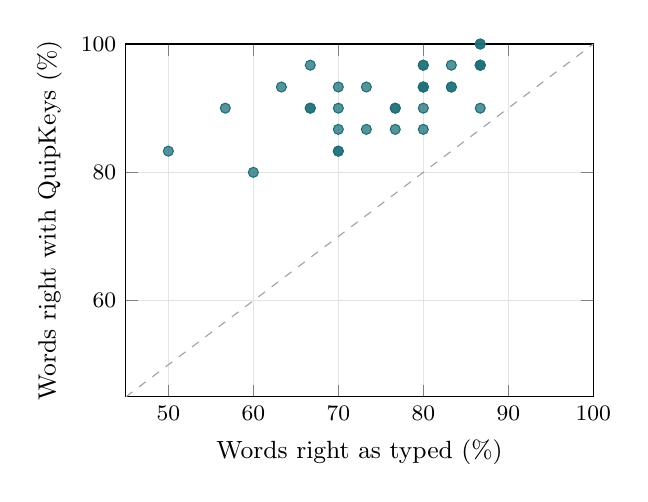
\begin{tikzpicture}
\begin{axis}[width=0.62\linewidth,height=0.5\linewidth,
  xlabel={Words right as typed (\%)},ylabel={Words right with \qk{} (\%)},
  xmin=45,xmax=100,ymin=45,ymax=100,grid=major,grid style={qkgrey!30},
  tick label style={font=\footnotesize},label style={font=\small}]
\addplot[qkgrey,dashed,domain=45:100] {x};
\addplot[only marks,mark=*,mark size=1.8pt,qkteal,fill opacity=0.75] coordinates {
(80.0,96.7) (80.0,93.3) (66.7,90.0) (83.3,93.3) (70.0,86.7) (80.0,93.3) (80.0,90.0) (76.7,90.0) (80.0,93.3) (50.0,83.3) (80.0,86.7) (70.0,83.3) (70.0,83.3) (76.7,86.7) (56.7,90.0) (86.7,100.0) (73.3,93.3) (86.7,96.7) (63.3,93.3) (80.0,96.7) (83.3,93.3) (70.0,93.3) (76.7,90.0) (73.3,86.7) (66.7,90.0) (86.7,96.7) (86.7,100.0) (86.7,90.0) (70.0,90.0) (83.3,96.7) (86.7,96.7) (60.0,80.0) (66.7,96.7)};
\end{axis}
\end{tikzpicture}
\caption{Real typing, one point per 30-word run (33 runs, 75--96 WPM, text hidden, no backspace). Every run lies above the diagonal.}
\label{fig:real}
\end{figure}

\begin{table}[t]
\centering\small
\caption{Real typing (33 runs, 990 words). ``Held-out'' is the 21 runs typed after the personal error model was fitted on the first 12.}
\label{tab:real}
\begin{tabular}{lcc}
\toprule
System & All 33 runs & Held-out 21 runs \\
\midrule
As typed & 75.4\% & 75.7\% \\
plain (frequency-only spellchecker) & 84.7\% & -- \\
\qk{}, no context & 87.6\% & -- \\
\qk{}, no boundary repair & 89.9\% & -- \\
\qk{}, pairs only (no trigrams) & 90.3\% & -- \\
\qk{}, word-by-word (no lattice) & 91.2\% & -- \\
\qk{}, no keyboard geometry & 91.6\% & -- \\
\textbf{\qk{}} & \textbf{91.5\%} & \textbf{92.4\%} \\
\textbf{\qk{} + fitted error model} & \textbf{92.5\%} & \textbf{93.0\%} \\
\bottomrule
\end{tabular}
\end{table}

\paragraph{Accuracy.} Table~\ref{tab:real} and Figure~\ref{fig:real} show the results. The share of words typed exactly right rose from 75.4\% to 91.5\%. Every run improved, and three reached 96--100\%. At the participant's median raw speed of 85~WPM, that is roughly 64 correct words per minute uncorrected versus 78 with \qk{}. Caps Lock recovery, added after the first 12 runs exposed the problem, lifted those 12 runs (five of them typed with Caps Lock on) from 83.3\% to 90.0\%.

\paragraph{The real error profile.} Table~\ref{tab:profile} compares the participant's slips with the simulator's assumptions. Two assumptions were wrong. First, most extra letters were \emph{not} neighbours of the keys around them (66 of 100 extra letters). Second, swapped pairs happened at the participant's normal pace (median inter-key interval of about 100--150~ms) rather than as sub-45~ms roll-overs. Consistent with this, keyboard geometry, the most valuable component on simulated data, contributed nothing measurable on real data (Table~\ref{tab:real}). Context and boundary repair carried the gains. An error model refitted to these frequencies (Table~\ref{tab:channel}) gained 1.7 points on the 12 runs it was fitted to and 0.6 points on the 21 runs typed afterwards.

\begin{table}[t]
\centering\small
\caption{Error profile of real typing (33 runs, 3,944 letters, 346 slips) versus the discrete-slip simulator.}
\label{tab:profile}
\begin{tabular}{lcc}
\toprule
Slip & Real typist & Simulator \\
\midrule
Wrong key & 32\% (71\% adjacent) & 40\% (90\% adjacent) \\
Missing letter & 22\% & 19\% \\
Extra letter, not near neighbours & 19\% & 0\% \\
Extra letter, adjacent or repeat & 10\% & 19\% \\
Swapped pair & 14\% & 22\% \\
Word boundary & 4\% & $\approx$10\% \\
\midrule
Letters mistyped & 8.8\% & 10\% (blind) \\
\bottomrule
\end{tabular}
\end{table}

\paragraph{What remains.} Of the 81 words still wrong across all runs, half are real-word slips (\ttw{ship} for \emph{shop}, \ttw{our}/\ttw{out}, \ttw{nice} for \emph{nine}, \ttw{quite}/\ttw{quiet}). Trigram context cannot overrule these safely. The other half are non-words with two or more slips or a genuinely ambiguous reading (\ttw{asn}: \emph{and} or \emph{an}? \ttw{thei}: \emph{this}, \emph{their} or \emph{the}?).

\subsection{Speed}
Median latency is 0.5--1.2~ms per word, and the 99th percentile is 3--10~ms, the upper end under rough aim. That is well below perceptible delay. The engine loads in about 1~s and compiles unchanged to WebAssembly for use in a browser.

\subsection{Negative results and lessons}
\label{sec:lessons}
\begin{itemize}
\item \textbf{4-grams.} Adding 6.6M 4-grams from the same 1.4B words gave no gain and more false corrections. They were dropped.
\item \textbf{A learned decision gate.} A logistic model over 18 decision features, trained with the evaluation's cost weights, improved its training objective. On the benchmark it raised false corrections enough to cancel the gain; restricted to non-word decisions it was roughly neutral, so it was not adopted.
\item \textbf{A neural language model.} A 23M-parameter word-level transformer trained for 3~hours on an RTX~2060 (400M words, validation perplexity 59) was used in two ways: as a left-context re-ranker of each chunk's readings, and as a look-ahead that rescores a real word's one-slip alternatives with the words that follow. On simulated typing it doubled real-word fixes (8\% to 17\%) but cost about a point overall, added false corrections, and was too slow (18~ms per word median in our unoptimised inference). On the participant's real typing it changed nothing: the words after a real-word slip are often misspelled themselves, and with a prior of about 7~nats against a one-slip real-word error, 2--4~nats of language-model evidence (e.g.\ \ttw{ate fat too much} vs.\ \ttw{far}) is correctly not enough. It is off by default.
\item \textbf{A document word cache} reinforced uncorrected slips and was replaced by learning only words typed identically twice.
\item \textbf{Dictionary hygiene matters.} A rule meant to admit UK/US variant pairs (\ttw{enrolment} and \ttw{enrollment}) also admitted 364 web misspellings (\ttw{actualy}, \ttw{realy}, \ttw{allready}), which the engine then treated as words. Real variants are within about 10$\times$ of each other in frequency; misspellings are 300--3000$\times$ rarer than the word they misspell. A frequency-ratio filter separates them cleanly. The participant's own typing (\ttw{actyaly}) exposed this bug, which the simulator never could.
\end{itemize}

\section{Limitations}
\label{sec:limits}
\begin{itemize}
\item \textbf{One participant.} The real-typing study has a single participant, who is also the author. The held-out split guards against fitting to particular runs, not to a particular typist.
\item \textbf{No comparison with operating-system autocorrect.} We could not run macOS or Windows autocorrect in our environment, so the baseline is our own frequency-only spellchecker.
\item \textbf{Effective speed versus careful typing is not yet measured.} The key behavioural question is whether fast, sloppy typing with \qk{} beats careful typing with backspace. The participant's careful baseline was not recorded.
\item \textbf{A simulator mismatch.} Simulated results are tuned to a simulator that real data showed to be partly wrong (Table~\ref{tab:profile}).
\item \textbf{Variety mismatch in evaluation.} The evaluation text is 1960s American prose, while the engine prefers UK spellings when correcting.
\item \textbf{No operating-system integration.} The system has not yet been integrated as an input method, where issues such as secure fields and application compatibility arise.
\end{itemize}

\section{Conclusion and Future Work}
\qk{} shows that the decoding approach that freed phone typists from precision transfers to physical keyboards. On real sloppy typing at 85~WPM, it raised exact-word accuracy from 75\% to over 91\%, while rarely touching correct text. Real data was decisive. It corrected the simulator, found a dictionary bug, and showed that context, not geometry, carries the gains for this typist.

The next steps are:
\begin{itemize}
\item measuring careful-typing and operating-system-autocorrect baselines on the same participant;
\item recruiting more typists, including people with motor impairments, for whom imprecision is not a choice;
\item stronger evidence for real-word slips, from longer look-ahead or a larger model;
\item learning each user's error profile online;
\item input-method integration on Windows and macOS.
\end{itemize}

\paragraph{Acknowledgements.} The engine, benchmark and this paper were developed with the help of Claude, an AI assistant by Anthropic.

\bibliographystyle{plainnat}
\bibliography{refs}

\end{document}
